\documentclass[8pt]{beamer}
\usepackage{listings}
\usetheme{Darmstadt}
\setbeamertemplate{footline}[frame number]
\usepackage{graphics}
\usepackage{pgf, tikz}
\usepackage{fancybox}
\usepackage{amssymb}
\usepackage{subcaption}
\usetikzlibrary{arrows, automata,calc}
\usetikzlibrary{er,positioning}
\title{Final Presentation of NII Internship}%Static Analysis for Reachability Problem
\author{Xinwei Chai}
\date{May 15, 2018}
% Macros relatives à la traduction de PH avec arcs neutralisants vers PH à k-priorités fixes

% Macros générales
%\newcommand{\ie}{\textit{i.e.} }
\newcommand{\segm}[2]{\llbracket #1; #2 \rrbracket}
%\newcommand{\f}[1]{\mathsf{#1}}

% Notations générales pour PH
\newcommand{\PH}{\mathcal{PH}}
%\newcommand{\PHs}{\mathcal{S}}
\newcommand{\PHs}{\Sigma}
%\newcommand{\PHp}{\mathcal{P}}
\newcommand{\PHp}{\textcolor{red}{\mathcal{P}}}
%\newcommand{\PHproc}{\mathcal{P}}
\newcommand{\PHproc}{\mathbf{Proc}}
\newcommand{\Proc}{\PHproc}
\newcommand{\PHh}{\mathcal{H}}
\newcommand{\PHa}{\PHh}
%\newcommand{\PHa}{\mathcal{A}}
\newcommand{\PHl}{\mathcal{L}}
\newcommand{\PHn}{\mathcal{N}}

\newcommand{\PHhitter}{\mathsf{hitter}}
\newcommand{\PHtarget}{\mathsf{target}}
\newcommand{\PHbounce}{\mathsf{bounce}}
%\newcommand{\PHsort}{\Sigma}
\newcommand{\PHsort}{\PHs}

%\newcommand{\PHfrappeur}{\mathsf{frappeur}}
%\newcommand{\PHcible}{\mathsf{cible}}
%\newcommand{\PHbond}{\mathsf{bond}}
%\newcommand{\PHsorte}{\mathsf{sorte}}
%\newcommand{\PHbloquant}{\mathsf{bloquante}}
%\newcommand{\PHbloque}{\mathsf{bloquee}}

%\newcommand{\PHfrappeR}{\textcolor{red}{\rightarrow}}
%\newcommand{\PHmonte}{\textcolor{red}{\Rsh}}

\newcommand{\PHhitA}{\rightarrow}
\newcommand{\PHhitB}{\Rsh}
%\newcommand{\PHfrappe}[3]{\mbox{$#1\PHhitA#2\PHhitB#3$}}
%\newcommand{\PHfrappebond}[2]{\mbox{$#1\PHhitB#2$}}
\newcommand{\PHhit}[3]{#1\PHhitA#2\PHhitB#3}
\newcommand{\PHfrappe}{\PHhit}
\newcommand{\PHhbounce}[2]{#1\PHhitB#2}
\newcommand{\PHobj}[2]{\mbox{$#1\PHhitB^*\!#2$}}
\newcommand{\PHobjectif}{\PHobj}
\newcommand{\PHconcat}{::}
%\newcommand{\PHneutralise}{\rtimes}
\def\Sce{\mathbf{Sce}}

% Actions plurielles
\newcommand{\PHhitmultsymbol}{\rightarrowtail}
\newcommand{\PHhitmult}[2]{\mbox{$#1 \PHhitmultsymbol #2$}}
\newcommand{\PHfrappemult}{\PHhitmult}
\newcommand{\PHfrappemults}[2]{\PHhitmult{\{#1\}}{\{#2\}}}

\def\PHget#1#2{{#1[#2]}}
%\newcommand{\PHchange}[2]{#1\langle #2 \rangle}
%\newcommand{\PHchange}[2]{(#1 \Lleftarrow #2)}
%\newcommand{\PHarcn}[2]{\mbox{$#1\PHneutralise#2$}}
\newcommand{\PHplay}{\cdot}

\newcommand{\PHstate}[1]{\mbox{$\langle #1 \rangle$}}
\newcommand{\PHetat}{\PHstate}

\def\supp{\mathsf{support}}
\def\first{\mathsf{first}}
\def\last{\mathsf{last}}

\def\DNtrans{\rightarrow_{ADN}}
\def\DNdef{(\mathbb F, \langle f^1, \dots, f^n\rangle)}
\def\DNdep{\mathsf{dep}}
\def\PHPtrans{\rightarrow_{PH}}
\def\get#1#2{#1[{#2}]}
\def\encodeF#1{\mathbf{#1}}
\def\toPH{\encodeF{PH}}
\def\card#1{|#1|}
\def\decode#1{\llbracket#1\rrbracket}
\def\encode#1{\llparenthesis#1\rrparenthesis}
\def\Hits{\PHa}
\def\hit{\PHhit}
\def\play{\cdot}

\def\Pint{\textsc{PINT}}



\usepackage{ifthen}

\newcommand{\currentScope}{}
\newcommand{\currentSort}{}
\newcommand{\currentSortLabel}{}
\newcommand{\currentAlign}{}
\newcommand{\currentSize}{}

\newcounter{la}
\newcommand{\TSetSortLabel}[2]{
  \expandafter\repcommand\expandafter{\csname TUserSort@#1\endcsname}{#2}
}
\newcommand{\TSort}[4]{
  \renewcommand{\currentScope}{#1}
  \renewcommand{\currentSort}{#2}
  \renewcommand{\currentSize}{#3}
  \renewcommand{\currentAlign}{#4}
  \ifcsname TUserSort@\currentSort\endcsname
    \renewcommand{\currentSortLabel}{\csname TUserSort@\currentSort\endcsname}
  \else
    \renewcommand{\currentSortLabel}{\currentSort}
  \fi
  \begin{scope}[shift={\currentScope}]
  \ifthenelse{\equal{\currentAlign}{l}}{
    \filldraw[process box] (-0.5,-0.5) rectangle (0.5,\currentSize-0.5);
    \node[sort] at (-0.2,\currentSize-0.4) {\currentSortLabel};
   }{\ifthenelse{\equal{\currentAlign}{r}}{
     \filldraw[process box] (-0.5,-0.5) rectangle (0.5,\currentSize-0.5);
     \node[sort] at (0.2,\currentSize-0.4) {\currentSortLabel};
   }{
    \filldraw[process box] (-0.5,-0.5) rectangle (\currentSize-0.5,0.5);
    \ifthenelse{\equal{\currentAlign}{t}}{
      \node[sort,anchor=east] at (-0.3,0.2) {\currentSortLabel};
    }{
      \node[sort] at (-0.6,-0.2) {\currentSortLabel};
    }
   }}
  \setcounter{la}{\currentSize}
  \addtocounter{la}{-1}
  \foreach \i in {0,...,\value{la}} {
    \TProc{\i}
  }
  \end{scope}
}

\newcommand{\TTickProc}[2]{ % pos, label
  \ifthenelse{\equal{\currentAlign}{l}}{
    \draw[tick] (-0.6,#1) -- (-0.4,#1);
    \node[tick label, anchor=east] at (-0.55,#1) {#2};
   }{\ifthenelse{\equal{\currentAlign}{r}}{
    \draw[tick] (0.6,#1) -- (0.4,#1);
    \node[tick label, anchor=west] at (0.55,#1) {#2};
   }{
    \ifthenelse{\equal{\currentAlign}{t}}{
      \draw[tick] (#1,0.6) -- (#1,0.4);
      \node[tick label, anchor=south] at (#1,0.55) {#2};
    }{
      \draw[tick] (#1,-0.6) -- (#1,-0.4);
      \node[tick label, anchor=north] at (#1,-0.55) {#2};
    }
   }}
}
\newcommand{\TSetTick}[3]{
  \expandafter\repcommand\expandafter{\csname TUserTick@#1_#2\endcsname}{#3}
}

\newcommand{\myProc}[3]{
  \ifcsname TUserTick@\currentSort_#1\endcsname
    \TTickProc{#1}{\csname TUserTick@\currentSort_#1\endcsname}
  \else
    \TTickProc{#1}{#1}
  \fi
  \ifthenelse{\equal{\currentAlign}{l}\or\equal{\currentAlign}{r}}{
    \node[#2] (\currentSort_#1) at (0,#1) {#3};
  }{
    \node[#2] (\currentSort_#1) at (#1,0) {#3};
  }
}
\newcommand{\TSetProcStyle}[2]{
  \expandafter\repcommand\expandafter{\csname TUserProcStyle@#1\endcsname}{#2}
}
\newcommand{\TProc}[1]{
  \ifcsname TUserProcStyle@\currentSort_#1\endcsname
    \myProc{#1}{\csname TUserProcStyle@\currentSort_#1\endcsname}{}
  \else
    \myProc{#1}{process}{}
  \fi
}

\newcommand{\repcommand}[2]{
  \providecommand{#1}{#2}
  \renewcommand{#1}{#2}
}
\newcommand{\THit}[5]{
  \path[hit] (#1) edge[#2] (#3#4);
  \expandafter\repcommand\expandafter{\csname TBounce@#3@#5\endcsname}{#4}
}
\newcommand{\TBounce}[4]{
  (#1\csname TBounce@#1@#3\endcsname) edge[#2] (#3#4)
}

%\newcommand{\TState}[1]{
%  \foreach \proc in {#1} {
%    \node[current process] (\proc) at (\proc.center) {};
%  }
%}

\newcommand{\TState}[1]{
  \foreach \proc in {#1} {
        \node[current process] (\proc) at (\proc.center) {};
  };
}
\newcommand{\TCoopHit}[6]{
  \node[#2, apdot] at (#3) {};
  \foreach \proc in {#1} {
    \draw[#2,-] (#3) edge (\proc);
  }
  \path[hit] (#3) edge[#2] (#4#5);
  \expandafter\repcommand\expandafter{\csname TBounce@#4@#6\endcsname}{#5}
}

% ex : \TAction{c_1}{a_1.west}{a_0.north west}{}{right}
% #1 = frappeur
% #2 = cible
% #3 = bond
% #4 = style frappe
% #5 = style bond
\newcommand{\TAction}[5]{
  \THit{#1}{#4}{#2}{}{#3}
  \path[bounce, bend #5=50] \TBounce{#2}{}{#3}{};
}

% ex : \TActionPlur{f_1, c_0}{a_0.west}{a_1.south west}{}{3.5,2.5}{left}
% #1 = frappeur
% #2 = cible
% #3 = bond
% #4 = style frappe
% #5 = coordonnées point central
% #6 = direction bond
\newcommand{\TActionPlur}[6]{
  \TCoopHit{#1}{#4}{#5}{#2}{}{#3}
  \path[bounce, bend #6=50] \TBounce{#2}{}{#3}{};
}

% procedure, abstractions and dependencies
\newcommand{\abstr}[1]{#1^\wedge}%\text{\textasciicircum}}
\def\BS{\mathbf{BSeq}}
\def\aBS{\abstr{\BS}}
\def\abeta{\abstr{\beta}}
\def\aZ{\abstr{\zeta}}
\def\aY{\abstr{\xi}}

\def\beforeproc{\vartriangleleft}

\def\powerset{\wp}

\def\Sce{\mathbf{Sce}}
\def\OS{\mathbf{OSeq}}
\def\Obj{\mathbf{Obj}}
%\def\Proc{\mathbf{Proc}}
%\def\Sol{\mathbf{Sol}}
\newcommand{\Sol}{\mathbf{Sol}}
\newcommand{\NSol}{\Sol}
\newcommand{\sSol}{\mathbf{Sync}}

\usepackage{galois}
\newcommand{\theOSabstr}{toOS}
\newcommand{\OSabstr}[1]{\theOSabstr(#1)}
\newcommand{\theOSconcr}{toSce}
\newcommand{\OSconcr}[1]{\theOSconcr(#1)}

% \def\gO{\mathbb{O}}
% \def\gS{\mathbb{S}}
\def\aS{\mathcal{A}}
\def\Req{\mathrm{Req}}
%\def\Sol{\mathrm{Sol}}
\def\Cont{\mathrm{Cont}}
\def\cBS{\BS_\ctx}
\def\caBS{\aBS_\ctx}
\def\caS{\aS_\ctx}
\def\cSol{\Sol_\ctx}
\def\cReq{\Req_\ctx}
\def\cCont{\Cont_\ctx}

\def\any{\star}

% \def\gProc{\mathrm{maxPROC}}
\def\mCtx{\mathrm{maxCtx}}

%\def\procs{\f{procs}}
\def\objs{\f{objs}}
\def\sat#1{\lceil #1\rceil}

\def\gCont{\f{maxCont}}
\def\lCont{\f{minCont}}
\def\lProc{\f{minProc}}
\def\gProc{\f{maxProc}}

\def\join{\oplus}
\def\concat{\!::\!}
\def\emptyseq{\varepsilon}
\def\ltw{\preccurlyeq_{\OS}}
\def\indexes#1{\mathbb{I}^{#1}}
%\def\indexes#1{\{1..|#1|\}}
\def\supp{\f{support}}
\def\w{\omega}
\def\W{\Omega}
% \def\ctx{\varsigma}
%\def\ctx{{\textcolor{green}{s}}}
% \def\ctx{s}
% \def\Ctx{\mathbf{Ctx}}
\def\Ctx{\mathbf{Ctx}}
\def\mconcr{\gamma}
\def\concr{\mconcr_s}
\def\obj#1#2{{#1\!\Rsh^*\!\!#2}}
\def\objp#1#2#3{\obj{{#1}_{#2}}{{#1}_{#3}}}
\def\A{\mathcal{A}}
\def\cwA{\A_\ctx^\w}
\def\cwReq{\Req_\ctx^\w}
\def\cwSol{\Sol_\ctx^\w}
\def\cwCont{\Cont_\ctx^\w}
\def\gCtx{\f{maxCtx}}
\def\endCtx{\f{endCtx}}
\def\ceil{\f{end}}

%\def\lfp{\mathrm{lfp}\;}
%\def\mlfp#1{\mathrm{lfp}\{#1\}\;}
\newcommand{\lfp}[3]{\mathbf{lfp}\{#1\}\left(#2\mapsto#3\right)}
\def\maxobjs{{\f{maxobjs}}}
\def\maxprocs{{\f{maxprocs}_\ctx}}
\def\objends{{\f{ends}}}

\def\ra{\rho}
\def\rb{\rho^\wedge}
\def\rc{\widetilde{\rho}}
\def\interleave{\f{interleave}}

\def\join{\concat}

\tikzstyle{aS}=[every edge/.style={draw,->,>=stealth}]
\tikzstyle{Asol}=[draw,circle,minimum size=5pt,inner sep=0,node distance=1cm]
\tikzstyle{Aproc}=[draw,node distance=1cm]
\tikzstyle{Aobj}=[node distance=1.5cm]
\tikzstyle{Anos}=[font=\Large]
\tikzstyle{Assol}=[node distance=1.2cm]
%\tikzstyle{AprocPrio}=[Aproc,double]
\tikzstyle{AsolPrio}=[Asol,double]
\tikzstyle{AprocPrio}=[Aproc,double]
\tikzstyle{aSPrio}=[aS,double]


\newcommand{\startl}[1]{\node[Aproc] (#1) {$#1$};\node[Asol,right of=#1] (#1s) {};\path (#1) edge (#1s);}%start link
\newcommand{\link}[2]{\node[Aproc,right of=#1s] (#2) {$#2$};\node[Asol,right of=#2] (#2s) {};\path (#1s) edge (#2) (#2) edge (#2s);} %normal link
\newcommand{\specl}[3]{\node[Aproc,#1 right of=#2s] (#3) {$#3$};\node[Asol,right of=#3] (#3s) {};\path (#2s) edge (#3) (#3) edge (#3s);} %special link
\newcommand{\edl}[2]{\node[Assol,right of=#1s] (#1st){$\varnothing$};\path (#1s) edge (#1st);}%end link


%\def\procs{\mathsf{procs}}
%\def\allprocs{\mathsf{allProcs}}
%\def\allprocs{\procs}
%\def\pfp{\mathsf{pfp}}
\def\pfp{\mathsf{focals}^1}
\def\pfpprocs{\mathsf{pfpProcs}}
\def\bounceprocs{\mathsf{bounceProcs}}
\def\newprocs{\mathsf{newProcs}}

\def\aB{\mathcal{B}}
\def\sat#1{{#1}}
%\def\sat#1{\lceil #1\rceil}
\newcommand{\thisB}[2]{\sat{\aB_{#2}^{#1}}}
\newcommand{\myp}{u}
%\def\cwB{\thisB{\myp}{\ctx}}
\def\cwB{\thisB{\myp}{s}}
%\def\cwB{\sat{\aB_\ctx^\w}}
%\def\cwBz{\thisB{\myp}{\ctx_0}}
\def\cwBz{\thisB{\myp}{s_0}}
\def\mycwB#1#2{\sat{\aB_{#1}^{#2}}}
\def\Bsol{\sat{\Sol^\w_\ctx}}
\def\Breq{\sat{\Req^\w_\ctx}}
\def\Bcont{\sat{\Cont^\w_\ctx}}

\def\myB{\aB^\myp_\ctx}
\def\mysol{\overline{\Sol^\w_\ctx}}
\def\myreq{\overline{\Req^\w_\ctx}}
\def\mycont{\overline{\Cont^\w_\ctx}}

\newcommand{\csState}{\mathsf{procState}}

\newcommand{\V}{V}
\newcommand{\E}{E}
\newcommand{\cwV}{\V_s^\myp}
\newcommand{\cwE}{\E_s^\myp}
% \newcommand{\cwV}{\V_\ctx^\myp}
% \newcommand{\cwE}{\E_\ctx^\myp}
%\newcommand{\VProc}{\textcolor{red}{\V_\PHproc}}
%\newcommand{\VObj}{\textcolor{red}{\V_\Obj}}
%\newcommand{\VSol}{\V_{Sol}}
%\newcommand{\VSol}{\textcolor{red}{\V_{\Sol}}}
\newcommand{\VProc}{\V \cap \PHproc}
\newcommand{\VObj}{\V \cap \Obj}
\newcommand{\VSol}{\V \cap \Sol}
\newcommand{\cwVProc}{\cwV \cap \PHproc}
\newcommand{\cwVObj}{\cwV \cap \Obj}
\newcommand{\cwVSol}{\cwV \cap \Sol}
\newcommand{\cwVsSol}{\cwV \cap \sSol}

\def\Bv{\sat{\cwV}}
\def\Be{\sat{\cwE}}
\def\BvProc{\textcolor{red}{\sat{\cwV}^\PHproc}}
\def\BvObj{\textcolor{red}{\sat{\cwV}^\Obj}}
%\def\BvSol{\sat{\cwV}^{Sol}}
\def\BvSol{\textcolor{red}{\sat{\cwV}^{\Sol}}}

\def\cwBNodes{\Bv}
\def\cwBEdges{\Be}
\def\nsol{\f{nsol}}
\def\conn{\f{conn}}

\newcommand{\Bee}[2]{\Be^{#1}_{#2}}

%\def\mlfp#1{\f{pppf}\{#1\}}

\def\PHobjp#1#2#3{\PHobj{{#1}_{#2}}{{#1}_{#3}}}
\def\Obj{\mathbf{Obj}}
\def\powerset{\wp}
\def\gCont{\f{maxCont}}

\def\muconcr{\ell}
\def\uconcr{\muconcr_\ctx}

% Styles TikZ et couleurs personnalisées

\usepackage{tikz}

\newdimen\pgfex
\newdimen\pgfem
\usetikzlibrary{arrows,shapes,shadows,scopes}
\usetikzlibrary{positioning}
\usetikzlibrary{matrix}
\usetikzlibrary{decorations.text}
\usetikzlibrary{decorations.pathmorphing}
\usetikzlibrary{arrows,shapes}

\definecolor{lightgray}{rgb}{0.8,0.8,0.8}
\definecolor{lightgrey}{rgb}{0.8,0.8,0.8}

\definecolor{lightred}{rgb}{1,0.8,0.8}
\definecolor{lightgreen}{rgb}{0.7,1,0.7}
\definecolor{darkgreen}{rgb}{0,0.5,0}
\definecolor{darkblue}{rgb}{0,0,0.5}
\definecolor{darkyellow}{rgb}{0.5,0.5,0}
\definecolor{lightyellow}{rgb}{1,1,0.6}
\definecolor{darkcyan}{rgb}{0,0.6,0.6}
\definecolor{lightcyan}{rgb}{0.6,1,1}
\definecolor{darkorange}{rgb}{0.8,0.2,0}
\definecolor{notsodarkred}{rgb}{0.8,0,0}

\definecolor{notsodarkgreen}{rgb}{0,0.7,0}

%\definecolor{coloract}{rgb}{0,1,0}
%\definecolor{colorinh}{rgb}{1,0,0}
\colorlet{coloract}{darkgreen}
\colorlet{colorinh}{red}
\colorlet{coloractgray}{lightgreen}
\colorlet{colorinhgray}{lightred}
\colorlet{colorinf}{darkgray}
\colorlet{coloractgray}{lightgreen}
\colorlet{colorinhgray}{lightred}

\colorlet{colorgray}{lightgray}
\colorlet{colorhl}{blue}


\tikzstyle{boxed ph}=[]
\tikzstyle{sort}=[fill=lightgray, rounded corners, draw=black]
\tikzstyle{process}=[circle,draw,minimum size=15pt,fill=white,font=\footnotesize,inner sep=1pt]
%\tikzstyle{black process}=[process, draw=blue, fill=red,text=black,font=\bfseries]
\tikzstyle{gray process}=[process, draw=black, fill=lightgray]
\tikzstyle{highlighted process}=[current process, fill=gray]
\tikzstyle{process box}=[fill=none,draw=black,rounded corners]
\tikzstyle{current process}=[process, draw=black, fill=lightgray]
%\tikzstyle{current process}=[process,fill=lightcyan]
\tikzstyle{hl process}=[process,fill=blue!30]
\tikzstyle{tick label}=[font=\footnotesize]
\tikzstyle{tick}=[densely dotted] %-
\tikzstyle{hit}=[->,>=angle 45]
\tikzstyle{selfhit}=[min distance=50pt,curve to]
\tikzstyle{bounce}=[densely dotted,>=stealth',->]
\tikzstyle{ulhit}=[draw=lightgray,fill=lightgray]
\tikzstyle{pulhit}=[fill=lightgray]
\tikzstyle{bulhit}=[draw=lightgray]
\tikzstyle{hl}=[very thick,colorhl]
\tikzstyle{hlb}=[very thick]
\tikzstyle{hlhit}=[hl]
%\tikzstyle{hl2}=[hl]
%\tikzstyle{nohl}=[font=\normalfont,thin]

\tikzstyle{update}=[draw,->,dashed,shorten >=.7cm,shorten <=.7cm]

\tikzstyle{unprio}=[draw,thin]%[double]
%\tikzstyle{prio}=[draw,thick,-stealth]%[double]
\tikzstyle{prio}=[draw,-stealth,double]

\tikzstyle{hitless graph}=[every edge/.style={draw=red,-}]

\tikzstyle{aS}=[every edge/.style={draw,->,>=stealth}]
\tikzstyle{Asol}=[draw,circle,minimum size=5pt,inner sep=0,node distance=1cm]
\tikzstyle{Aproc}=[draw,node distance=1.2cm]
\tikzstyle{Aobj}=[node distance=1.5cm]
\tikzstyle{Anos}=[font=\Large]

\tikzstyle{AsolPrio}=[Asol,double]
\tikzstyle{AprocPrio}=[Aproc,double]
\tikzstyle{aSPrio}=[aS,double]

\colorlet{colorhlwarn}{notsodarkred}
\colorlet{colorhlwarnbg}{lightred}
\tikzstyle{Ahl}=[very thick,fill=colorhlwarnbg,draw=colorhlwarn,text=colorhlwarn]
\tikzstyle{Ahledge}=[very thick,double=colorhlwarnbg,draw=colorhlwarn,color=colorhlwarn]





%\definecolor{darkred}{rgb}{0.5,0,0}



\tikzstyle{grn}=[every node/.style={circle,draw=black,outer sep=2pt,minimum
                size=15pt,text=black}, node distance=1.5cm, ->]
\tikzstyle{inh}=[>=|,-|,draw=colorinh,thick, text=black,label]
\tikzstyle{act}=[->,>=triangle 60,draw=coloract,thick,color=coloract]
\tikzstyle{inhgray}=[>=|,-|,draw=colorinhgray,thick, text=black,label]
\tikzstyle{actgray}=[->,>=triangle 60,draw=coloractgray,thick,color=coloractgray]
\tikzstyle{inf}=[->,draw=colorinf,thick,color=colorinf]
%\tikzstyle{elabel}=[fill=none, above=-1pt, sloped,text=black, minimum size=10pt, outer sep=0, font=\scriptsize,draw=none]
\tikzstyle{elabel}=[fill=none,text=black, above=-2pt,%sloped,
minimum size=10pt, outer sep=0, font=\scriptsize, draw=none]
%\tikzstyle{elabel}=[]


\tikzstyle{plot}=[every path/.style={-}]
\tikzstyle{axe}=[black,->,>=stealth']
\tikzstyle{ticks}=[font=\scriptsize,every node/.style={black}]
\tikzstyle{mean}=[thick]
\tikzstyle{interval}=[line width=5pt,red,draw opacity=0.7]
%\definecolor{lightred}{rgb}{1,0.3,0.3}

%\tikzstyle{hl}=[yellow]
%\tikzstyle{hl2}=[orange]

%\tikzstyle{every matrix}=[ampersand replacement=\&]
%\tikzstyle{shorthandoff}=[]
%\tikzstyle{shorthandon}=[]
\tikzstyle{objective}=[process,very thick,fill=yellow!50]

\tikzstyle{coopupdate}=[-stealth,decorate,decoration={zigzag,amplitude=1.5pt,post=lineto,post length=.3cm,pre=lineto,pre length=.3cm}]

\tikzstyle{labelprio}=[circle, fill=blue!30, inner sep=0pt, minimum size=13pt]
\tikzstyle{labelprio1}=[labelprio]
\tikzstyle{labelprio2}=[labelprio, fill=red!60]
\tikzstyle{labelprio3}=[labelprio, fill=orange!50]
\tikzstyle{labelprio4}=[labelprio, fill=brown!50]

\tikzstyle{labelstocha}=[rectangle, rounded corners=4pt]

\tikzstyle{andot}=[circle, fill=black, inner sep=1.2pt, draw=transparent]
\tikzstyle{anligne}=[thick]

\tikzstyle{apdot}=[andot] %[circle, fill=black, draw=black, inner sep=1]
\tikzstyle{apdotsimple}=[] %[circle, fill=black, draw=black, inner sep=1]

% Figure de résumé des liens entre les formalismes
\tikzstyle{equiv-externe}=[thick, rounded corners, draw=gray, fill=gray!10, align=center,
  inner sep=8]

% label pour les délais des actions 
 \tikzstyle{labeldelai1}=[circle, fill=red!60, inner sep=0pt, minimum size=8pt]
  \tikzstyle{labeldelai2}=[circle, fill=blue!30, inner sep=0pt, minimum size=8pt]
  \tikzstyle{labeldelai3}=[circle, fill=brown!50, inner sep=0pt, minimum size=8pt]
  \tikzstyle{labeldelai4}=[circle, fill=green!50, inner sep=0pt, minimum size=8pt]
  
% Automata Networks:
\tikzstyle{local transitions}=[->,>=latex',thick,bend left=30,
               every node/.style={fill=white,inner sep=1pt,outer sep=1pt}]
\tikzstyle{reach}=[fill=lightgray,ellipse]

\tikzstyle{local transitions 2}=[->,>=latex',thick,bend left=100,
               every node/.style={fill=white,inner sep=1pt,outer sep=4pt}]

\tikzstyle{local transitions 3}=[->,>=latex',thick,bend right=100,
               every node/.style={ right, fill=white,inner sep=1pt,outer sep=4pt}]
               
% Graphe d'états
% noeuds
\tikzstyle{vide}= [rectangle, minimum width=2em,minimum height=1.5em,]
\tikzstyle{stable}= [rectangle,fill=lightred]
\tikzstyle{current}= [rectangle,fill=lightcyan]
\tikzstyle{initial}= [rectangle,fill=green!20]

% % STG transitions
\tikzstyle{etiquette}=[midway,fill=blue!20,circle,scale=0.7pt]
\tikzstyle{etiquette2}=[midway,fill=green!20,circle,scale=0.7pt]
%
\tikzstyle{currentTrans}=[->,very thick,blue]
\tikzstyle{seperatedTransPart1}=[draw, thick, blue]
\tikzstyle{seperatedTransPart2}=[->, thick, blue]


\tikzstyle{mytext}=[thick, text width=4.5em,inner sep=1pt]
\tikzstyle{line} =[draw, thick, -latex',shorten >=2pt]
\tikzstyle{block} =[rectangle,text width=6em,draw,minimum height=4em, outer sep=0pt]

\tikzstyle{adn}=[every node/.style={circle,draw=black,outer sep=2pt,minimum
                size=15pt,text=black}, node distance=1.5cm, ->]
                
% Définition des nouvelles options xmin, xmax, ymin, ymax
% Valeurs par défaut : -3, 3, -3, 3
\tikzset{
    xmin/.store in=\xmin, xmin/.default=-3, xmin=-3,
    xmax/.store in=\xmax, xmax/.default=3, xmax=3,
    ymin/.store in=\ymin, ymin/.default=-3, ymin=-3,
    ymax/.store in=\ymax, ymax/.default=3, ymax=3,
}
% Commande qui trace la grille entre (xmin,ymin) et (xmax,ymax)
\newcommand {\grille}
    {\draw[help lines] (\xmin,\ymin) grid (\xmax,\ymax);}
% Commande \axes
\newcommand {\axes} {
    \draw[->] (\xmin,0) -- (\xmax+0.5,0);
    \draw[->] (0,\ymin) -- (0,\ymax+0.5);
}
% Commande qui limite l’affichage à (xmin,ymin) et (xmax,ymax)
\newcommand {\fenetre}
    {\clip (\xmin,\ymin) rectangle (\xmax,\ymax);}
   
 \newcommand{\nombresCopiesParNote}
   {(0,0)(1,0)(2,2)(3,0)(4,6)(5,4)(6,7)(7,4)(8,3)(9,0)(10,1)}  
% Expression level of a
 \newcommand{\expressionDiscreteA}
   {(0,0)(1,0)(2,0)(3,0)(4,0)(4,1)(5,1)(5,0)(6,0)(7,0)(8,0)(9,0)(9,1)(10,1)(11,1)(12,1)(13,1)(13,0)(14,0)(15,0)(16,0)(17,0)(17,1)(18,1)}      
   
% Expression level of b
 \newcommand{\expressionDiscreteB}
   {(0,1)(12,1)(12,0)(18,0)} 
   
% Expression level of z
 \newcommand{\expressionDiscreteZ}
   {(0,0)(3,0)(3,1)(14,1)(14,0)(18,0)}
\tikzstyle{block} = [rectangle, draw, fill=blue!20, 
    text width=6em, text centered, rounded corners, minimum height=4em]
    \tikzstyle{line} = [draw, -latex']

\newcommand{\libcirc}[1]{\pgfmathparse{
    ifthenelse(#1 > 0 && #1 < 21, Hex(9311+#1), Hex(9450)
    }\libertineGlyph{uni\pgfmathresult}}
\begin{document}
\maketitle
\begin{frame}{About His Research}
\begin{itemize}
\item A 3rd-year PhD student from Laboratory of digital sciences of Nantes (LS2N), France, co-working with Tony, supervised by Morgan Magnin, Olivier Roux
\end{itemize}
\begin{columns}
\begin{column}{.5\textwidth}
\centering
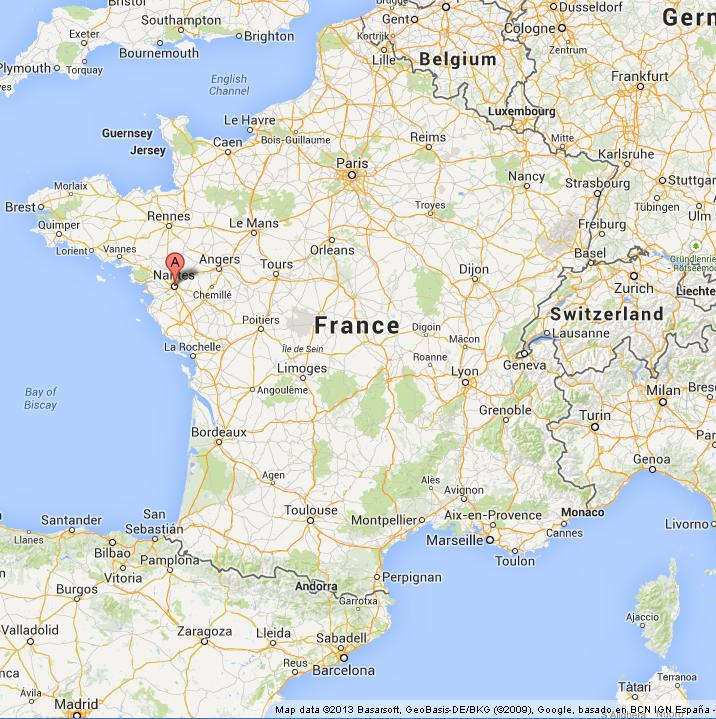
\includegraphics[scale=0.27]{Nantes.jpg}
\end{column}
\begin{column}{.5\textwidth}
\begin{itemize}
\item Research topics:
\begin{itemize}
\item Dynamical modelings% of biological regulatory network
\item Analysis of dynamical properties (Model checking)
\item Answer Set Programming (declarative programming)
\item LFIT, Neuron Network (Model inference)
\end{itemize}
\end{itemize}

\end{column}
\end{columns}
\end{frame}

\begin{frame}{Outline}
\begin{columns}
\begin{column}{0.7\textwidth}
    \begin{figure}
       \centering
       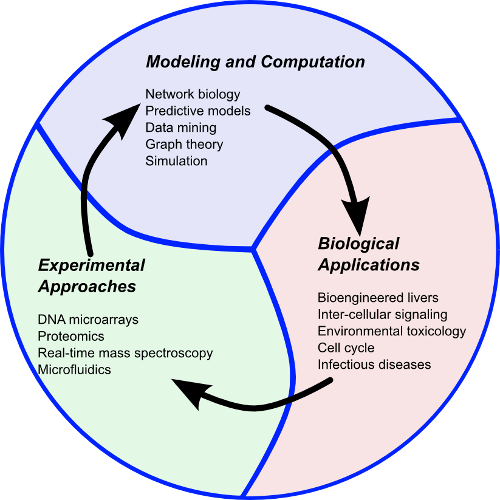
\includegraphics[height=0.7\paperheight]{systems_biology.png}
   \end{figure}
\end{column}
\begin{column}{0.3\textwidth}
%More precisely:
    \only<2>{
    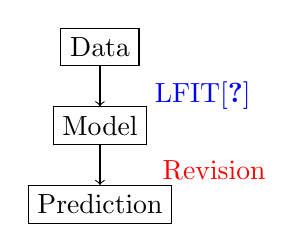
\begin{tikzpicture}
        \node [draw](data) {Data};
        \node [draw,below of = data] (model) {Model};
        \draw[->] (data) -- (model);
        \node [draw,below of = model] (pred) {Prediction};
        \draw[->] (model) -- (pred);
        \node [below right = 0.1cm of data] (LFIT){\textcolor{blue}{LFIT\cite{ribeiro2013bdd}}};
        \node [below right = 0.1cm of model] (Revision){\textcolor{red}{Revision}};
    \end{tikzpicture}
    }
\end{column}
\end{columns}
\end{frame}
\begin{frame}{Process Scheme}
\begin{figure}
    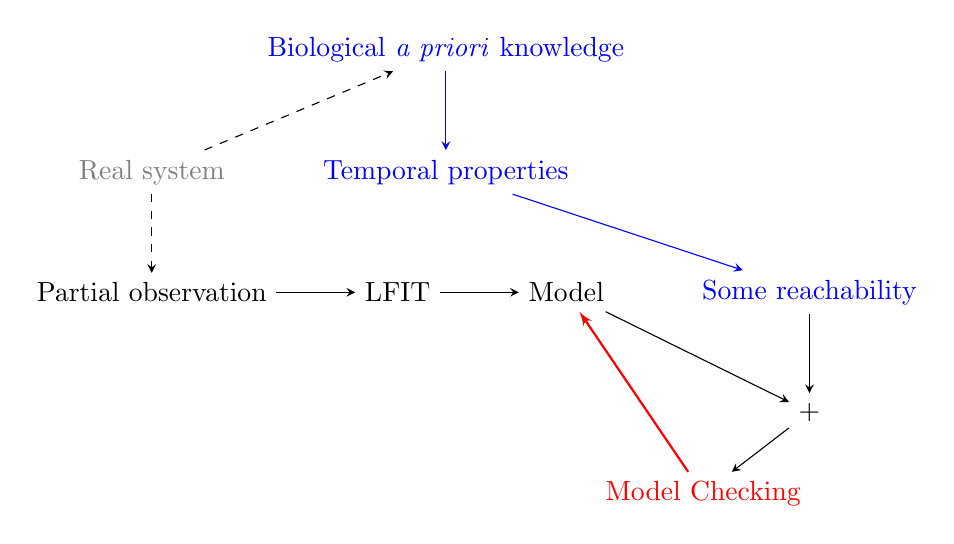
\begin{tikzpicture}[line,>=stealth]
        \node [color=gray] (1) {Real system};
        \node [color=blue,right = of 1] (2) {Temporal properties};
        \node [below = of 1] (3) {Partial observation};
        \node [right = of 3] (4) {LFIT};
        \node [right = of 4] (8) {Model};
        \draw [->] (4) -- (8);
        \node [color=blue,right = of 8] (5) {Some reachability};
        \node [color = red, below left = 2cm and -1.5cm of 5] (7) {Model Checking};
        \node [color=blue,above = of 2] (6) {Biological \textit{a priori} knowledge};
        \draw [dashed,->] (1) -- (6);
        \draw [color=blue,->] (2) -- (5);
        \draw [dashed,->] (1) -- (3);
        \draw [->] (3) -- (4);
        %\draw [->] (8) -- (5);
        \draw [color=blue, ->] (6) -- (2);
        \node [below = of 5] (9) {$+$};
        \draw [->] (8) --(9);
        \draw [->] (5) --(9);
        \draw [->] (9) --(7);
        \draw[thick, color=red] (7)--(8);
    \end{tikzpicture}
\end{figure}
    
\end{frame}

\begin{frame}{Table of Contents}
    \tableofcontents
\end{frame}

\section{Modeling framework}% \& static analysis}
\begin{frame}{Models \& Semantics}
\begin{columns}

\begin{column}{.3\textwidth}
%\begin{tikzpicture}
%\node at (0,0) {a};
%\node at (2.2,0) {b};
%\node at (1,1.1){+};
%\node at (1,-1.1){$-$};
%\draw[->] (5pt,5pt) .. controls (0.67,1) and (1.33,1) .. (2,5pt);
%\draw[->] (2,-5pt) .. controls  (1.33,-1)and (0.67,-1) .. (5pt,-5pt);
%\end{tikzpicture}

%Regulatory network


$$a(t+1)= \lnot b(t)$$
$$b(t+1)=a(t)$$

Boolean Network

\begin{figure}
    \centering
    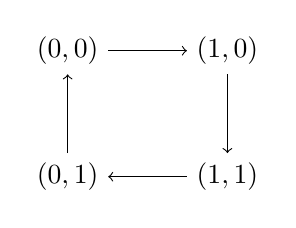
\begin{tikzpicture}
\node (00) {$(0,0)$};
\node [below = 1cm of 00] (01) {$(0,1)$};
\node [right = 1cm of 01] (11) {$(1,1)$};
\node [right = 1cm of 00] (10) {$(1,0)$};
\draw[->] (00) -- (10);
\draw[->] (10) -- (11);
\draw[->] (11) -- (01);
\draw[->] (01) -- (00);

\end{tikzpicture}
    \caption{State transition graph}
    \label{fig:my_label}
\end{figure}
\end{column}
\begin{column}{.1\textwidth}
$\Longrightarrow$
\vspace{3.5cm}
\end{column}
\begin{column}{.5\textwidth}
\textcolor{blue}{\textit{body}\hspace{0.5cm}  \textit{head}}

$\{b_0\}\to a_0 \Rsh a_1,\ \{b_1\}\to a_1 \Rsh a_0,$
$\{a_0\}\to b_1 \Rsh b_0,\ \{a_1\}\to b_0 \Rsh b_1$
\begin{figure}
    \centering
    \begin{tikzpicture}[apdotsimple/.style={apdot}]

\TSort{(0,0)}{a}{2}{l}
\TSort{(2.5,0)}{b}{2}{l}

\path[local transitions]

	(a_0) edge node[auto] {$b_0$} (a_1)
	(b_0) edge node[auto] {$a_1$} (b_1)
    (a_1) edge node[auto] {$b_1$} (a_0)
    (b_1) edge node[auto] {$a_0$} (b_0)
;

\TState{a_0, b_0}
\end{tikzpicture}

    \caption{Automata network}
\end{figure}

%\vspace{0.5cm}
%States of the system $(a,b)$: (0,0), (0,1), (1,0), (1,1)
\end{column}
\end{columns}
%\vspace{0.5cm}
% Asynchronous Automata Network (AAN):

\end{frame}

\section{Reachability analysis}
\begin{frame}{Reachability problem}
\begin{columns}
	\begin{column}{.5\textwidth}
	\begin{figure}
    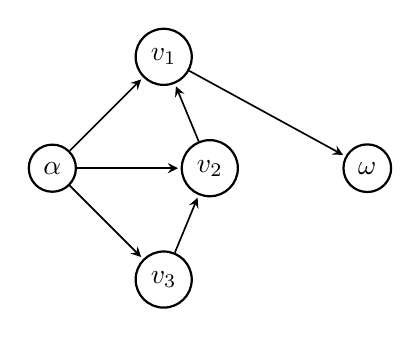
\begin{tikzpicture}[
            > = stealth, % arrow head style
            shorten > = 1pt, % don't touch arrow head to node
            auto,
            node distance = 2cm, % distance between nodes
            semithick % line style
        ]

        \tikzstyle{every state}=[
            draw = black,
            thick,
            fill = white,
            minimum size = 4mm
        ]

        \node[state] (s) {$\alpha$};
        \node[state] (v1) [above right of=s] {$v_1$};
        \node[state] (v2) [right of=s] {$v_2$};
        \node[state] (v3) [below right of=s] {$v_3$};
        \node[state] (t) [right of=v2] {$\omega$};

        \draw[->] (s) -- (v1);
        \draw[->] (s) -- (v2);
        \draw[->] (s) -- (v3);
        \draw[->] (v2) -- (v1);
        \draw[->] (v3) -- (v2);
        \draw[->] (v1) -- (t);

    \end{tikzpicture}
    \caption{State transition graph} 
    \end{figure}
    \end{column}
    \begin{column}{.5\textwidth}
    Given a Boolean Network, from initial state $\alpha$, does there exist a transition sequence that reaches the target state $\omega$?

    \vspace{0.25cm}
%\begin{center}
%    $\Updownarrow$
%\end{center}
{\centering $\Updownarrow$

}
    
    
    \vspace{0.25cm}
   
   
    Given a state transition graph, from initial state $\alpha$, does there exist a pathway towards the target state $\omega$?
    \end{column}
\end{columns}

\vspace{0.1cm}

The size of state transition graph is of $O(val^n)$, with $val$ the number of possible values of automata and $n$ the number of automata

\vspace{0.1cm}

Reachability of global states \fbox{$\mathbf{EF}(a_i,b_j,\ldots)$} is usually computationally difficult and unnecessary to analyze, thus it is preferred to study partial reachability problem \fbox{$\mathbf{EF}a_i$}

\end{frame}



\begin{frame}{Difficulties and solution}
\begin{itemize}
\item State space grows exponentially with the number of automata
\item Traditional model checkers e.g. Mole\footnote{\url{http://www.lsv.fr/~schwoon/tools/mole}} and NuSMV\footnote{\url{http://nusmv.fbk.eu}} fail

global search $\to$ time out and/or out of memory
\item \textbf{Static analysis}: avoid global search, at the cost of precision
\end{itemize}
$\to$ A balance between time-space performance and conclusiveness
\vspace{0.25cm}
\begin{itemize}
    \item Paulev\'e \textit{et al.} introduced LCG (Local Causality Graph) \cite{folschette2015,pauleve2012} for static analysis
    \item Implementation: Pint
\end{itemize}

\begin{itemize}
    \item Efficient (beats many traditional model checkers) \textbf{but}
    \item Usually not conclusive when the sparsity of the biological network increases
\end{itemize}
\end{frame}

\begin{frame}{Local Causality Graph (LCG)}
What is LCG?

A static analytic structure

\vspace{0.5cm}
Start with target state $\omega\to$ Find transitions reaching $\omega\to$ Find new target states to fire those transitions $\to\cdots$ Recursion $\cdots\to$ End with initial state $\alpha$

\begin{itemize}
\item Goal-oriented structure 
\item Formed by recursive updates
%starting with desired final state, for each update, link the states with their associated transitions if they are not at initial state. Update ends when the graph becomes saturated.
\item Avoid global search in state transition graphs
\end{itemize}

\end{frame}


%\begin{frame}{Algorithm for Reachability}
%    \begin{itemize}
%    \item Input: An Automata Network $A$ and 2 partial states $init, target$ 
%    \item Output: \textbf{UNREACHABLE, REACHABLE, INCONCLUSIVE}
%\end{itemize}
%\begin{enumerate}
%    \item Construct the LCG $\ell=LCG(A,target)$
%    \item Check pseudo-reachability, can return \textbf{UNREACHABLE}
%    \item Clean all cycles and prune $\ell$
%    \item \textcolor{blue}{
%     Try at most $k$ times}
%    \begin{itemize}
%    \item \textcolor{blue}{$\ell'\gets \ell$}
%    \item \textcolor{blue}{ Transform randomly each OR gate $O$ of $\ell'$ into simple gate}
%    \item\textcolor{blue}{ Generate all trajectories $t$ to reach $target$ in $\ell$ using ASP}
%    \begin{itemize}
%        \item\textcolor{blue}{ If a valid $t$ is found, return \textbf{REACHABLE}}
%    \end{itemize}
%    \end{itemize}
%    \item\textcolor{blue}{ return \textbf{INCONCLUSIVE}}
%\end{enumerate}
%\end{frame}


\begin{frame}{Construction of LCG}
\begin{figure}
\begin{tikzpicture}
\TSort{(0,0)}{a}{2}{l}
\TSort{(2,0)}{b}{2}{l}
\TSort{(4,0)}{c}{2}{l}
\TSort{(6,0)}{d}{2}{l}
\TSort{(8,0)}{e}{2}{l}

% with delays
\path[local transitions]

	(d_0) edge node[auto] {\textcolor<10>{red}{$\{b_1$\}}} (d_1)
    (a_0) edge[bend left] node[auto] {\textcolor<3,5,6>{red}{$\{b_1,c_1\}$}} (a_1)
    (a_0) edge[bend right] node[right] {\textcolor<2,4>{red}{$\{e_1$\}}} (a_1)
    (b_0) edge[bend left] node[auto] {\textcolor<7>{red}{$\{d_0\}$}} (b_1)
	(c_0) edge node[auto] {\textcolor<8>{red}{$\{d_1\}$}} (c_1)
%	(d_0) edge node[auto] {$b_1$} (d_1)
	%(c_1) edge node[auto] {$\{b_0\}$, $2$} (c_0)
	%(c_0) edge node[auto] {$d_1$} (c_1)
;

\TState{a_0, b_0, c_0, d_0,e_0}


\end{tikzpicture}
\end{figure}

\begin{figure}

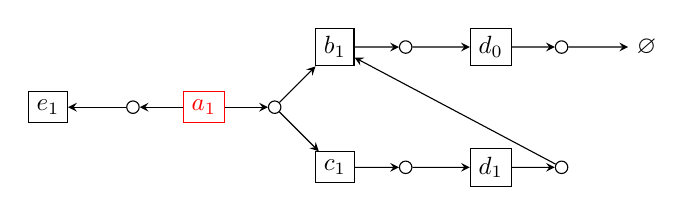
\begin{tikzpicture}[aS,scale=0.9, every node/.style={scale=0.9}]  
  	\onslide<1-10>{\node[color=red,Aproc] (a_1) {$a_1$};}
  	\onslide<3-10>{\node[Asol,right of=a_1] (a_1s) {};}
  	\onslide<3-10>{\path (a_1) edge (a_1s);}
  	%\onslide<10-12>{\node[right = 0.1cm of a_1s] {\textcolor<10>{red}{AND}};}
  	%\onslide<11-12>{\node[above = 0.1cm of a_1] {\textcolor<11>{red}{OR}};}
    \onslide<2-10>{\node[Asol,left of=a_1] (a_1s1){};}
    \onslide<4-10>{\node[Aproc,left of=a_1s1] (e_1){$e_1$};}
    \onslide<4-10>{\path (a_1s1) edge (e_1);}
    \onslide<2-10>{\path(a_1) edge (a_1s1);}
  	\onslide<5-10>{\specl{above}{a_1}{b_1};}
  	\onslide<7-10>{\link{b_1}{d_0};}
  	\onslide<9-10>{\edl{d_0};}
  	\onslide<6-10>{\specl{below}{a_1}{c_1};}
	\onslide<8-10>{\link{c_1}{d_1};}
    \onslide<10-10>{\path (d_1s) edge (b_1);}
\end{tikzpicture}


\end{figure}
Small circles stand for transition nodes, squares for state nodes

\only<6>{$r'(a_1)=r'(e_1)\lor (r'(b_1)\land r'(c_1)$)}
\only<7>{$r'(a_1)=r'(d_0)\land r'(c_1)$}
\only<8>{$r'(a_1)=r'(d_0)\land r'(d_1)$}
\only<9>{$r'(a_1)=r'(d_1)$}
\only<10>{$r'(a_1)=r'(b_1)=r'(d_0)=1$}
\end{frame}

\begin{frame}{Algorithm for Reachability}
    \begin{itemize}
    \item Input: An Automata Network $A$ and 2 states $\alpha, \omega$ 
    \item Output: \textbf{UNREACHABLE, REACHABLE, INCONCLUSIVE}
\end{itemize}
\begin{enumerate}
    \item \textcolor{gray}{Construct the LCG $\ell=LCG(A,\alpha,\omega)$}
    \item \textcolor{gray}{Check pseudo-reachability, can return \textbf{UNREACHABLE}}
    \item Clean all cycles and prune $\ell$
    \item \textcolor{blue}{Try at most $k$ times}
    \begin{itemize}
        \item {$\ell'\gets \ell$}
        \item { Transform randomly each OR gate $O$ of $\ell'$ into simple gate}
        \item \textcolor{blue}{ Generate all trajectories $t$ to reach $target$ in $\ell$ using ASP}
        \begin{itemize}
            \item\textcolor{blue}{If a valid $t$ is found, return \textbf{REACHABLE}}
        \end{itemize}
    \end{itemize}
    \item\textcolor{blue}{return \textbf{INCONCLUSIVE}}
\end{enumerate}
\end{frame}

%\begin{frame}{Heuristics at OR gates}
%Make random decision at each OR gate $\to$
%
%An LCG without OR gates
%\begin{figure}
%\begin{tikzpicture}[level/.style={sibling distance=45mm/#1},scale=0.8]
\node [circle,draw] (z){$t$}
  child {node [circle,draw,fill=gray] (a) {}
    child {node [circle,draw,fill=gray] (b) {}
      child {node {$\vdots$}
        child {node [circle,draw] (d) {}}
        child {node [circle,draw,fill=gray] (e) {}}
      } 
      child {node {$\vdots$}}
    }
    child {node [circle,draw] (g) {}
      child {node {$\vdots$}}
      child {node (mid) {$\vdots$}}
    }
  }
  child {node [circle,draw] (j) {}
    child {node [circle,draw] (k) {}
      child {node {$\vdots$}}
      child {node {$\vdots$}}
    }
  child {node [circle,draw] (l) {}
    child {node {$\vdots$}}
    child {node (c){$\vdots$}
      child {node [circle,draw] (o) {}}
      child {node [circle,draw] (p) {}
        child [grow=right] {node (q) {} edge from parent[draw=none]
          child [grow=right] {node (q) {} edge from parent[draw=none]
            child [grow=up] {node (r) {} edge from parent[draw=none]
              child [grow=up] {node (s) {} edge from parent[draw=none]
                child [grow=up] {node (t) {} edge from parent[draw=none]
                  child [grow=up] {node (u) {} edge from parent[draw=none]}
                }
              }
            }
            child [grow=down] {node (v) {}edge from parent[draw=none]}
          }
        }
      }
    }
  }
};
\node [right = 2.3cm of e] (point){$\cdots$};
\path (a) -- (j) node [midway] {};
\path (b) -- (g) node [midway] {};
\path (k) -- (l) node [midway] {};
\path (k) -- (g) node [midway] {};
\path (d) -- (e) node [midway] {};
\path (o) -- (p) node [midway] {};
\path (o) -- (e) node (x) [midway] {}
  child [grow=down] {
    node (y) {}
    edge from parent[draw=none]
  };
\path (q) -- (r) node [midway] {};
\path (s) -- (r) node [midway] {};
\path (s) -- (t) node [midway] {};
\path (s) -- (l) node [midway] {};
\path (t) -- (u) node [midway] {};
\path (z) -- (u) node [midway] {};
\path (j) -- (t) node [midway] {};
\path (y) -- (x) node [midway] {};
\path (v) -- (y)
  node (w) [midway] {};
\path (q) -- (v) node [midway] {};
\path (e) -- (x) node [midway] {};
\path (o) -- (x) node [midway] {};
\path (y) -- (w) node [midway] {};
\path (v) -- (w) node [midway] {};
\path (r) -- (c) node [midway] {};
\end{tikzpicture}
%\end{figure}
%\end{frame}

\begin{frame}{Reasoning with LCG}
LCG is \textbf{exact} for unreachability 

LCG is \textbf{exact} when it does not contain self-dependent structure:
\begin{itemize}


\item different state nodes of the same automaton in different branches:
\end{itemize}
Given initial state: $a_0,b_0,c_0$, consider the reachability of $c_1$:
\begin{figure}
    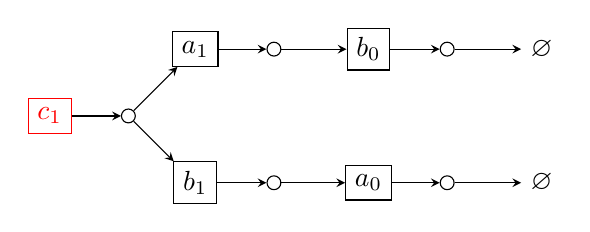
\begin{tikzpicture}[aS]  
  	
  	  	\node[color=red,Aproc] (c_1) {$c_1$};\node[Asol,right of=c_1] (c_1s) {};\path (c_1) edge (c_1s);
  	\specl{above}{c_1}{a_1};
  	\link{a_1}{b_0};
  	\edl{b_0};
  	\specl{below}{c_1}{b_1};
	\link{b_1}{a_0};
  	\edl{a_0};
    \end{tikzpicture}

\end{figure}

Reaching $a_1$ disables the reachability of $b_1$, and vice versa, $c_1$ is unreachable
\end{frame}

%\begin{frame}{Deleting cycles in LCG}
%\begin{figure}
%    \centering
%    \begin{tikzpicture}

\def \n {6}
\def \radius {2cm}
\def \margin {8} % margin in angles, depends on the radius


\node[draw] at ({360/\n * 2}:\radius) (x) {$x$};
\invisible<4>{\node[draw, circle, minimum size=6pt, inner sep = 0] at ({360/\n * 3}:\radius) {};}
\invisible<4>{\node[draw] at ({360/\n * 4}:\radius) (y) {$y$};}
\only<1,2,5>{\node[draw, circle, minimum size=6pt, inner sep = 0] at ({360/\n * 5}:\radius) {};
\node[draw] at ({360/\n * 6}:\radius) (z) {$z$};}
\only<1,5>{\node[draw, circle, minimum size=6pt, inner sep = 0] at ({360/\n * 1}:\radius) {};
\foreach \s in {1,...,\n}
{
  
  \draw[->, >=latex] ({360/\n * (\s - 1)+\margin}:\radius) 
    arc ({360/\n * (\s - 1)+\margin}:{360/\n * (\s)-\margin}:\radius);
}}
\only<2>{\foreach \s in {3,...,\n}
{
  
  \draw[->, >=latex] ({360/\n * (\s - 1)+\margin}:\radius) 
    arc ({360/\n * (\s - 1)+\margin}:{360/\n * (\s)-\margin}:\radius);
}}
\only<3>{\foreach \s in {3,...,4}
{
  
  \draw[->, >=latex] ({360/\n * (\s - 1)+\margin}:\radius) 
    arc ({360/\n * (\s - 1)+\margin}:{360/\n * (\s)-\margin}:\radius);
}}

\node[left = 1.3cm of x, draw, circle, minimum size=6pt, inner sep = 0] (sol) {};
\node[left = 1.3cm of sol, draw] (origin) {$\omega$};
\draw[->, >=latex] (origin) to [bend left] (sol);
\draw[->, >=latex] (sol) to [bend left] (x);
\only<5>{\node[below = 1.7cm of origin, draw, circle, minimum size=6pt, inner sep = 0] (soly2) {};
\draw[->, >=latex] (origin) to [bend right] (soly2);
\draw[->, >=latex] (soly2) to [bend right] (y);
\invisible<4>{\draw[->, >=latex] (sol) to [bend right= 45] (z);}}
\end{tikzpicture}
%    \caption{
%    \only<1>{Cycle detection}
%    \only<2>{Break last link}
%    \only<3>{Delete useless part}
%    \only<4>{Delete useless part, $\omega$ is not reachable}
%    \only<5>{Unbreakable case $\to$ Inconclusive}}
%\end{figure}
%\end{frame}

%\begin{frame}{Cycles}
%The reachability of all components in a cycle are equal:
%$a_i\to\circ\to \cdots \to\circ\to a_i$
%
%$reach(a_i)=reach(a_i.\mathtt{next})=\cdots=reach(a_i)$
%
%\vspace{0.5cm}
%
%For a cycle containing no solution branches, all its components are unreachable (circular reasoning), otherwise their reachability is equal to the disjunction of the branches.
%
%\vspace{0.5cm}
%
%%After second preconditioning, %we obtain an acyclic LCG without OR gates.
%\end{frame}
\begin{frame}{Branches at transition nodes}
\begin{figure}
%\begin{tikzpicture}[apdotsimple/.style={apdot},scale=0.7, every node/.style={scale=0.8}]
\begin{tikzpicture}
\TSort{(0,0)}{a}{2}{l}
\TSort{(2.5,0)}{b}{2}{l}
\TSort{(5,0)}{c}{2}{l}
%\TSort{(7.5,0)}{d}{2}{l}
%\TSort{(10,0)}{e}{2}{l}

% with delays
\path[local transitions]

	(c_0) edge node[auto] {\{$a_1, b_1$\}} (c_1)
    (a_0) edge[bend left] node[auto] {$b_0$} (a_1)
	(b_0) edge node[auto] {$\mathbf{c_0}$} (b_1)
%	(d_0) edge node[auto] {$b_1$} (d_1)
	%(c_1) edge node[auto] {$\{b_0\}$, $2$} (c_0)
	%(c_0) edge node[auto] {$d_1$} (c_1)
;

%\TState{a_0, b_0, c_0, d_0,e_0}
\TState{a_0, b_0, c_0}


\end{tikzpicture}

\end{figure}
\begin{figure}
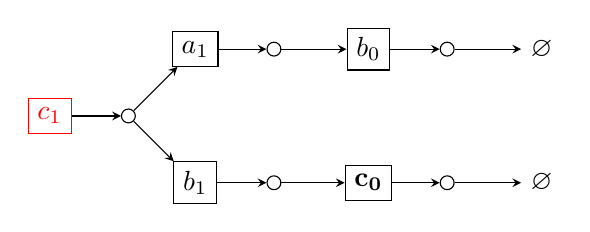
\begin{tikzpicture}[aS]
  	\node[color=red,Aproc] (c_1) {$c_1$};
  	\node[Asol,right of=c_1] (c_1s) {};
  	\path (c_1) edge (c_1s);
  	\specl{above}{c_1}{a_1};
  	\link{a_1}{b_0};
  	\edl{b_0};
  	\specl{below}{c_1}{b_1};
  	\node[Aproc,right of=b_1s] (c_0) {$\mathbf{c_0}$};
  	\path (b_1s) edge (c_0);
  	\node[Asol,right of=c_0] (c_0s) {};
  	\path (c_0) edge (c_0s);
  	\edl{c_0};
    \end{tikzpicture}

\end{figure}
\begin{table}[t]
    \centering
    \begin{tabular}{ccc}
        Admissible order:& $a_1\to b_1\to c_1$ &$\bigcirc$\\
        Impossible order:& $b_1\to a_1\to c_1$ &$\times$
    \end{tabular}
\end{table}

\end{frame}


\begin{frame}{Main contribution: Solution \textit{via} Answer Set Programming (ASP)}
Analyzer: ASPReach
\begin{itemize}
    \item Using declarative programming instead of imperative programming
    \item Describing the problem by rules and search coherent instances 
\end{itemize}

Semantics:

$$a_0\ \text{:-}\ a_1 ,\ \ldots,\ a_m,\ not\ a_{m+1},\ \ldots ,\ not\ a_n.$$    

$a_0$ is called \textit{head} and $a_1\ldots a_n$ is called \textit{body}

A transition $a_1\to b_0\Rsh b_1$ can be represented as: $b_1\ \text{:-}\ a_1,\ b_0$
\end{frame}
\begin{frame}{ASPReach}
In an LCG, link $a_1\to\circ\to b_1$ can be translated as: 

\texttt{node('a','1',1). node('b','1',2). parent(1,2).}

\vspace{0.5cm}

Core code:
\vspace{0.5cm}

\texttt{
\begin{tabular}{ll}
prior(N1,N2) :- &parent(N2,N1). \%Rule 1\\
prior(N1,N3) :- &prior(N1,N2), prior(N2,N3). \%Rule 2\\
prior(N1,N2) :- &node(P1,S1,N1), node(P2,S2,N2), \\
&node(P2,S3,N3), parent(N1,N3),\\
& init(P2,S3), S2!=S3, P1!=P2.\%Rule 3
\end{tabular}}

\vspace{0.5cm}
\texttt{N} for node, \texttt{P} for component, \texttt{S} for state

Rule 3: in the LCG, one branch contains $a_1\to\circ\to b_0$, another branch contains $b_1$, if $b_0\in \alpha$, $a_1$ is to be reached before reaching $b_1$

\end{frame}

\begin{frame}{Example}
\begin{figure}
%\begin{tikzpicture}[apdotsimple/.style={apdot},scale=0.7, every node/.style={scale=0.8}]
\begin{tikzpicture}
\TSort{(0,0)}{a}{2}{l}
\TSort{(2.5,0)}{b}{2}{l}
\TSort{(5,0)}{c}{2}{l}
%\TSort{(7.5,0)}{d}{2}{l}
%\TSort{(10,0)}{e}{2}{l}

% with delays
\path[local transitions]

	(c_0) edge node[auto] {\{$a_1, b_1$\}} (c_1)
    (a_0) edge[bend left] node[auto] {$b_0$} (a_1)
	(b_0) edge node[auto] {$\mathbf{c_0}$} (b_1)
%	(d_0) edge node[auto] {$b_1$} (d_1)
	%(c_1) edge node[auto] {$\{b_0\}$, $2$} (c_0)
	%(c_0) edge node[auto] {$d_1$} (c_1)
;

%\TState{a_0, b_0, c_0, d_0,e_0}
\TState{a_0, b_0, c_0}


\end{tikzpicture}

\end{figure}
\begin{figure}
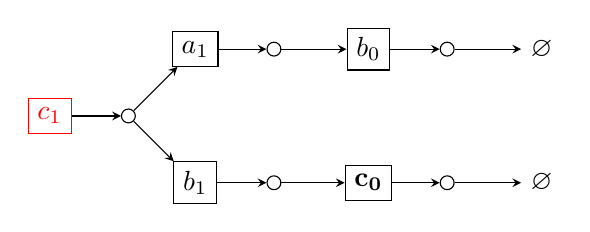
\begin{tikzpicture}[aS]
  	\node[color=red,Aproc] (c_1) {$c_1$};
  	\node[Asol,right of=c_1] (c_1s) {};
  	\path (c_1) edge (c_1s);
  	\specl{above}{c_1}{a_1};
  	\link{a_1}{b_0};
  	\edl{b_0};
  	\specl{below}{c_1}{b_1};
  	\node[Aproc,right of=b_1s] (c_0) {$\mathbf{c_0}$};
  	\path (b_1s) edge (c_0);
  	\node[Asol,right of=c_0] (c_0s) {};
  	\path (c_0) edge (c_0s);
  	\edl{c_0};
    \end{tikzpicture}

\end{figure}
$a\rhd b$ means $a$ appears in the sequence before $b$
\begin{tabular}{lll}
Rule 1 \& 2 &$\Rightarrow$& $b_0\rhd a_1\rhd c_1$ , $c_0 \rhd b_1\rhd c_1$\\
Rule 3 &$\Rightarrow$& $a_1 \rhd b_1$
\end{tabular}


The only admissible order is $a_1\to b_1\to c_1$
\end{frame}

\begin{frame}{Algorithm for Reachability}
    \begin{itemize}
    \item Input: An Automata Network $A$ and 2 states $\alpha, \omega$ 
    \item Output: \textbf{UNREACHABLE, REACHABLE, INCONCLUSIVE}
\end{itemize}
\begin{enumerate}
    \item \textcolor{gray}{Construct the LCG $\ell=LCG(A,\alpha,\omega)$}
    \item \textcolor{gray}{Check pseudo-reachability, can return \textbf{UNREACHABLE}}
    \item Clean all cycles and prune $\ell$
    \item \textcolor{blue}{Try at most $k$ times}
    \begin{itemize}
        \item {$\ell'\gets \ell$}
        \item { Transform randomly each OR gate $O$ of $\ell'$ into simple gate}
        \item \textcolor{blue}{ Generate all trajectories $t$ to reach $target$ in $\ell$ using ASP}
        \begin{itemize}
            \item\textcolor{blue}{If a valid $t$ is found, return \textbf{REACHABLE}}
        \end{itemize}
    \end{itemize}
    \item\textcolor{blue}{return \textbf{INCONCLUSIVE}}
\end{enumerate}
\end{frame}

\begin{frame}{Benchmark}
Traditional model checkers: Mole NuSMV $\to$ \textbf{memory-out}

Pure static analyzer: Pint \cite{folschette2015}

Small example: $\lambda$-phage, 4 components

Big examples: TCR (T-Cell Receptor, 95 components) and

EGFR (Epidermal Growth Factor Receptor, 106 components)

\small
\begin{table}[t]
    \centering
    \begin{tabular}{|c|c|c|c|c|c|c|}
    \hline
  	Model	&\multicolumn{2}{c|}{$\lambda$-phage}	&	  \multicolumn{2}{c|}{TCR} & \multicolumn{2}{c|}{EGFR}  \\
    \hline
    Inputs&\multicolumn{2}{c|}{4}	&	  \multicolumn{2}{c|}{3} & \multicolumn{2}{c|}{13}\\
    \hline
    Outputs&\multicolumn{2}{c|}{4} &	  \multicolumn{2}{c|}{5} & \multicolumn{2}{c|}{12} \\
    \hline
    Total tests&\multicolumn{2}{c|}{$2^4\times 4=64$} & \multicolumn{2}{c|}{$2^3\times 5=40$} & \multicolumn{2}{c|}{$2^{13}\times 12=98,304$}\\
    \hline
    Analyzer  &  Pint       &\textbf{ASPReach}    &  Pint       &\textbf{ASPReach}   &  Pint       &\textbf{ASPReach}             \\
    \hline
    Reachable    & 36(56\%)& 38(59\%)   &  \multicolumn{2}{c|}{16(40\%)}  & 64,282(65.4\%)&74,268(75.5\%)\\
    \hline
    \textbf{Inconclusive} & \textcolor{red}{\textbf{2(3\%)}}&\textcolor{blue}{\textbf{0(0\%)}}& \multicolumn{2}{c|}{0(0\%)}    &\textcolor{red}{\textbf{9,986(10.1\%)}}&\textcolor{blue}{\textbf{0(0\%)}}  \\
    \hline
    Unreachable     &  \multicolumn{2}{c|}{26(41\%)} &  \multicolumn{2}{c|}{24(60\%)} &24,036(24.5\%)&24,036(24.5\%)\\
    \hline
    Total runtime &  $<1$s       &  $<1$s &  \textbf{7s}       &  \textbf{0.85s}        & \textbf{9h50min}              & \textbf{3h46min}      \\
    \hline
    \end{tabular}
\end{table}


\end{frame}

\begin{frame}{Tests on Random Models}
\begin{columns}
    \begin{column}{0.65\textwidth}
        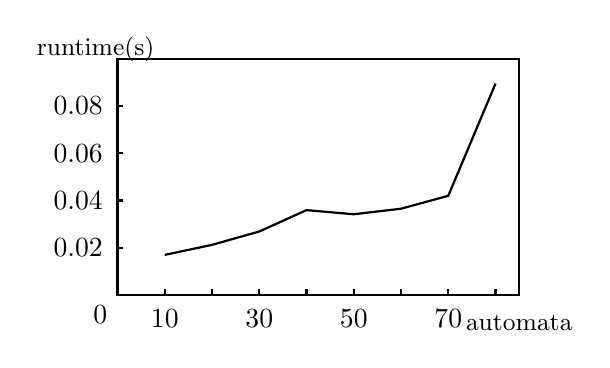
\begin{tikzpicture}[>=stealth,scale=0.6,line width=0.8pt]

% % % % % % % % % % % % % % %
 
\pgfmathsetmacro{\ticker}{0.125} 
 
\coordinate [label=225:0](A) at (0,0);
\coordinate (B) at (0,5);
\coordinate (C) at (8.5,5);
\coordinate (D) at (8.5,0);
\draw(A)--(B)--(C)--(D)--cycle;
 
\coordinate [label=left:{\small runtime(s)}](E) at ($(B)+(1,0.2)$);
\coordinate [label=below:{\small automata}](F) at ($(D)+(0,-0.2)$);
 
\foreach \i/\texti in {10,30,...,70} {
\draw (0.1*\i,0) --(0.1*\i,\ticker) node[label=below:\texti]{};
}
\foreach \i in {20,40,...,80} {
\draw (0.1*\i,0) --(0.1*\i,\ticker);
}

\foreach \j/\textj  in {0.02,0.04,0.06,0.08} {
\draw (0,50*\j) --(\ticker,50*\j) node[label=left:\textj]{};
}


\coordinate (1) at (1,6.8/8);
\coordinate (2) at (2,8.5/8);
\coordinate (3) at (3,10.76/8);
\coordinate (4) at (4,14.38/8);
\coordinate (5) at (5,13.68/8);
\coordinate (6) at (6,14.62/8);
\coordinate (7) at (7,16.8/8);
\coordinate (8) at (8,35.8/8);
\draw(1)--(2)--(3)--(4)--(5)--(6)--(7)--(8);
 
 
 
\end{tikzpicture}

        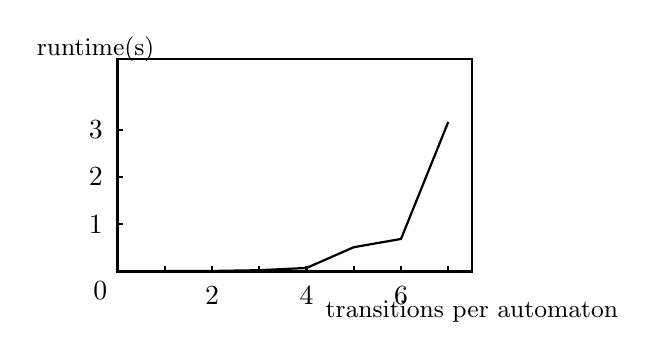
\begin{tikzpicture}[>=stealth,scale=0.6,line width=0.8pt,align=center]

% % % % % % % % % % % % % % %
 
\pgfmathsetmacro{\ticker}{0.125} 
 
\coordinate [label=225:0](A) at (0,0);
\coordinate (B) at (0,4.5);
\coordinate (C) at (7.5,4.5);
\coordinate (D) at (7.5,0);
\draw(A)--(B)--(C)--(D)--cycle;
 
\coordinate [label=left:{\small runtime(s)}](E) at ($(B)+(1,0.2)$);
\coordinate [label=below:{\small transitions per automaton}](F) at ($(D)+(0,-0.4)$);
 
\foreach \i/\texti in {2,4,...,7} {
\draw (\i,0) --(\i,\ticker) node[label=below:\texti]{};
}
\foreach \i in {20,60,...,140} {
\draw (0.05*\i,0) --(0.05*\i,\ticker);
}

\foreach \j/\textj  in {1,...,3} {
\draw (0,\j) --(\ticker,\j) node[label=left:\textj]{};
}


\coordinate (1) at (1,3.57/400);
\coordinate (2) at (2,3.9/400);
\coordinate (3) at (3,10.4/400);
\coordinate (4) at (4,29.4/400);
\coordinate (5) at (5,205/400);
\coordinate (6) at (6,275/400);
\coordinate (7) at (7,1265/400);
\draw(1)--(2)--(3)--(4)--(5)--(6)--(7);
 
 
 
\end{tikzpicture}

    \end{column}
    \begin{column}{0.35\textwidth}
        The top figure shows the average runtime increases with the number of automata with fixed sparsity (3 transitions per automaton). 
        We also carried tests on 1000 automata, the average runtime is bound in 3s. 
        
        \vspace{1cm}
        
        The bottom figure shows the runtime increases drastically with the transitions per automaton with the number of automaton fixed.
        Inconclusive cases appears after 7 transitions per automaton because the search space for every local state increases.
    \end{column}
\end{columns}
        
\end{frame}
\section{Model Revision}
\begin{frame}{Collaboration with LFIT}


\begin{itemize}
    \item If the model is consistent with \textit{a priori} knowledge
    \begin{itemize}
        \item Do nothing
    \end{itemize}
    \item If not consistent
    \end{itemize}
    \begin{table}[t]
        \centering
        \begin{tabular}{c|c|c}
            &Reachable &Unreachable\\
            \hline
            Knowledge& \multicolumn{1}{c}{$R_K$} & \multicolumn{1}{c}{$U_K$} \\
            \hline
            Inferred model& \multicolumn{1}{c}{$R_I$} & \multicolumn{1}{c}{$U_I$}\\
            \hline
            Inconsistency (problem)& $R'_K=R_K\cap U_I$ & $U'_K=R_I\cap U_K$\\
            Keep consistent with& $U_K$& $R_K$\\
            \hline
            Operation &Generalization$\bigcirc$ & Specialization$\bigcirc$\\
            &Add transitions$\times$&Delete transitions$\times$
            %$\checkmark$  
        \end{tabular}
    \end{table}
    
    where set $R$ and $U$ are consisting of pairs in the form $(\alpha, \omega)$
\end{frame}

\begin{frame}{Definitions}
\begin{block}{Specialization of a transition}
By adding elements in the body of a transition, it is possible to change a reachable state to an unreachable one
\end{block}
\begin{block}{Generalization of a transition}
By deleting elements in the body of a transition, it is possible to change an unreachable state to a reachable one
\end{block}
%\begin{block}{Adjacent pair}
%Data at two adjacent time points time series is called an instance.
%\end{block}
%\begin{block}{Inconsistency}
%If one instance is not consistent with \textit{a priori} knowledge, we have to revise \textit{a priori} knowledge. Thanks to asynchronous semantics, we do not have to check the consistency with the observations in most of the situations.
%\end{block}
\end{frame}

\begin{frame}{Main Algorithm}
    \begin{itemize}
        \item Input: an Automata Network $A$, reachable set $R_K$, unreachable set $U_K$
        \item Output: modified Automata Network $A$ or $\varnothing$ if not revisable
    \end{itemize}
    \begin{enumerate}
        \item Construct the LCGs for the elements in $R_K$ and $U_K$, collect inconsistent instances in set $R'_K$ and $U'_K$
        \item Specialize the transitions to make elements in $U'_K$ unreachable, if not possible, return $\varnothing$
        \item Generalize the transitions to make elements in $R'_K$ reachable, if not possible, return $\varnothing$
        \item Return $A$
    \end{enumerate}
\end{frame}

\begin{frame}{Specialization}
    \begin{itemize}
        \item Input: an Automata Network $A$, reachable set $R_K$, unreachable set $U_K$, inconsistent set $U'_K$
        \item Output: modified Automata Network $A$ or $\varnothing$ if not revisable
    \end{itemize}
    \begin{enumerate}
        \item Let set $L=\{\ell_i,\ldots\}$, $\ell_i=\{i,j,\ldots\}$, with $i\in U'_K$, $j\in LCG(i)$ and $ j\in R_K\cup U_K $ 
        \item Traverse $\ell_i\in L$ from the smallest cardinality, $\ell_i$ of size 1 can be directly revised from root as they do not have constraint of reachability
        \item For other in $\ell_i\in L$, check first their consistency, they may be already consistent because of the operation to $\ell_i$ of size 1
        \item Revise the remaining $\ell_i\in L$ from root $i$, if the revision is inconsistent with knowledge, revise the successor of $i$
        \item If there is no revision for $\ell_i$, return $\varnothing$
        %\item For $i$ in $R_K\cup U_K\cup L$
        %\begin{itemize}
        %    \item Create list $i$
        %    \item If $j\in LCG(i)$ with $j \in R_K\cup U_K$
        %    \begin{itemize}
        %        \item $i.next\gets i.next\cup j$
        %    \end{itemize}
        %\end{itemize}
        \item Return $A$
    \end{enumerate}
    Generalization is done analogously.
\end{frame}


\begin{frame}{Example: Specialization}
    Suppose initial state $\alpha=\langle a_0,b_0,c_0,d_0\rangle$, target state $\omega=a_1$, $U_K=\{(\alpha,a_1),(\alpha,c_1)\}$, $R_K=\{(\alpha,b_1)\}$
    \begin{figure}
        \centering
        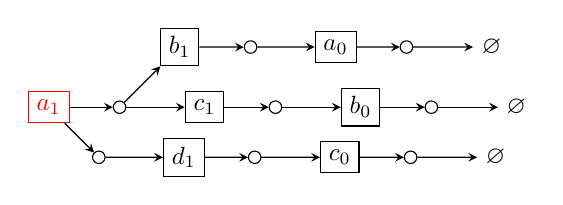
\begin{tikzpicture}[aS,scale=0.9, every node/.style={scale=0.9}]  
  	\node[color=red,Aproc] (a_1) {$a_1$};
  	\node[Asol,right  of = a_1] (a_1s) {};
  	\node[Asol,below right  of = a_1] (a_1s2) {};
  	\path (a_1) edge (a_1s);
  	\path (a_1) edge (a_1s2);
  	\node[Aproc,right of = a_1s2] (d_1) {$d_1$};
  	\node[Asol,right of = d_1] (d_1s) {};
  	\path (a_1s2) edge (d_1) (d_1) edge (d_1s);
  	\link{d_1}{c_0};
  	\edl{c_0};
  	\specl{above}{a_1}{b_1};
  	\link{b_1}{a_0};
 	\edl{a_0};
	\link{a_1}{c_1};
	\link{c_1}{b_0};
 	\edl{b_0};
\end{tikzpicture}
    \end{figure}
    The revision is computed as follows: 
    \begin{itemize}
        \item $L=\{\{(\alpha,a_1),(\alpha,c_1)\},\{(\alpha,c_1)\}\}$
        \item Revise $(\alpha,c_1)$ by $\{\mathbf{a_1}, b_0\}\to c_0\Rsh c_1$
        \item Check the reachability of $a_1$, $a_1$ is reachable due to path $a_1\to\circ\to d_1$
        \item Revise $(\alpha,a_1)$ by $\{\mathbf{a_1},c_0\}\to d_0\Rsh d_1$
        \item Check the reachability of $a_1$ and $c_1$, they are unreachable, finish
        %\item $\libcirc{1}\{b_1,c_1\}\to a_0\Rsh a_1,\libcirc{2}\{d_1\}\to a_0\Rsh a_1\}$
        %\item \libcirc{1} can be replaced by $\libcirc{3}\{a_0\}\to b_0\Rsh b_1\lor \libcirc{4}\{b_0\}\to c_0\Rsh c_1$
        %\item \libcirc{2} can be replaced by $\libcirc{5}\{c_0\}\to d_0\Rsh d_1$
    \end{itemize}
    %The only possible solution is to specialize \libcirc{4} and \libcirc{5}. We cannot specialize \libcirc{3} as $(\alpha,b_1)\in R_K$. Thus the solution is $\libcirc{4}'\{a_1, b_0\}\to c_0\Rsh c_1\land\libcirc{5}'\{a_1,c_0\}\to d_0\Rsh d_1\lor \{b_1,c_0\}\to d_0\Rsh d_1$
    
\end{frame}

\begin{frame}{Example: Generalization}
    Suppose initial state $\alpha=\langle a_0,b_0,c_0,d_0\rangle$, target state $\omega=a_1$, $U_K=\{(\alpha,c_1),(\alpha,d_1)\}$, $R_K=\{(\alpha,a_1)\}$
    \begin{figure}
        \centering
        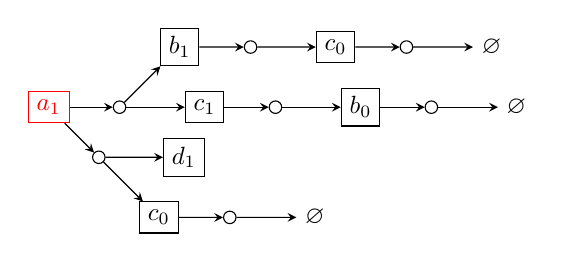
\begin{tikzpicture}[aS,scale=0.9, every node/.style={scale=0.9}]  
  	\node[color=red,Aproc] (a_1) {$a_1$};
  	\node[Asol,right of = a_1] (a_1s) {};
  	\node[Asol,below right of = a_1] (a_1s2) {};
  	\path (a_1) edge (a_1s);
  	\path (a_1) edge (a_1s2);
  	\node[Aproc,right of = a_1s2] (d_1) {$d_1$};
  	\node[Aproc,below right of = a_1s2] (c_0) {$c_0$};
  	\node[Asol,right of = c_0] (c_0s) {};
  	\path (a_1s2) edge (d_1);
  	\path (a_1s2) edge (c_0);
  	\path (c_0) edge (c_0s);
  	\edl{c_0};
  	\specl{above}{a_1}{b_1};
  	\link{b_1}{c_0};
 	\edl{c_0};
	\link{a_1}{c_1};
	\link{c_1}{b_0};
 	\edl{b_0};
\end{tikzpicture}
    \end{figure}
    The revision is computed as follows: 
    \begin{itemize}
        \item $L=\{\{(\alpha,a_1)\}\}$
        \item $a_1$ is reachable if (1)$\{b_1,c_1\}\to a_0\Rsh a_1$ or (2)$\{c_0,d_1\}\to a_0\Rsh a_1$ is generalized
        \item (1) can only be generalized to $\{b_1\}\to a_0\Rsh a_1$ as $c_1\in U_K$
        \item (2) can only be generalized to $\{c_0\}\to a_0\Rsh a_1$ as $d_1\in U_K$
        \item Check the reachability of $a_1$, reachable, finish
        %\item $\libcirc{1}\{b_1,c_1\}\to a_0\Rsh a_1,\libcirc{2}\{c_0,d_1\}\to a_0\Rsh a_1\}$
        %\item \libcirc{1} can be replaced by $\libcirc{3}\{c_0\}\to b_0\Rsh b_1\land \libcirc{4}\{b_0\}\to c_0\Rsh c_1$
    \end{itemize}
    %The solution is to specialize \libcirc{1} or \libcirc{2}. We cannot specialize \libcirc{4} as $(\alpha,c_1)\in U_K$. Thus the solution is $\libcirc{1}'\{b_1\}\to a_0\Rsh a_1\lor \libcirc{2}'\{c_0\}\to a_0\Rsh a_1$
    
\end{frame}

\begin{frame}{Conclusion}
    \begin{itemize}
        \item Developed model checker ASPReach, more efficient than traditional model checkers and more conclusive than pure static model checkers
        \item Given background knowledge (dynamic properties), we manage to revise the learned models with the help of LCG which make the learned models closer to reality
    \end{itemize}
    
    Ongoing work:
    \begin{itemize}
        \item Application in biological networks, \textit{e.g.} mammalian circadian clock modeling
    \end{itemize}
\end{frame}

%\begin{frame}{Case 1: Reachable $\to$ Unreachable}
%\begin{block}{Specialization via new instances}
%For asynchronous dynamics, only instances with new bodies can deny existing rules.
%\end{block}
%
%\begin{itemize}
%    \item Asynchronous Boolean network with components $a,b,c$, $a_1\gets b_1$ is inferred from $a_1,b_1,c_1\gets a_0,b_1,c_1$, and no $a_0,b_1,c_0$ is never observed in body
%
%    Specialization: instance $a_0,b_1,c_1\gets a_0,b_1,c_0$ denies the former rule and thus modify it to $a_1 \gets b_1\land c_1$%, also, $c_1$ is called ``modifiable''
%\end{itemize}
%
%Consider the incorporation with LCG, if by modifying transition $a_1\gets b_1$ to $a_1 \gets b_1\land c_1$ can make target unreachable, $c_1$ is said modifiable:
%
%Rule $a_1\gets b_1$, if we want $reach(a_1)=False$, $ reach(b_1)=True$
%
%Specialization: $a_1\gets b_1\land c_1$ where $c_1\in U_k\cap U_I$ 
%
%\begin{itemize}
%    \item If we believe the whole observation is perfect, it is not possible to delete one rule
%    \item Keep consistent with $R_K$
%\end{itemize}
%\end{frame}
%
%\begin{frame}{Case 2: Unreachable $\to$ Reachable}
%\begin{itemize}
%    \item Add rule with bodies in $R_k\cap R_I$ which do not subsume and which are not subsumed by any existing rule
%    
%    Existing rule: $a_1\gets b_1$, we do not add $a_1\gets $ or $a_1\gets b_1\land c_1$
%    \item Generalize a rule:
%
%$a_1\gets b_1\land c_1$, if we have $a_1\gets b_1\land c_0$, rule can be generalized to $a_1\gets b_1$
%
%\item Keep consistent with $U_K$
%
%\end{itemize}
%
%When it comes to LCG, Rule $a_1\gets b_1\land c_1$, if we want $reach(a_1)=True$, $reach(c_1)=False$
%
%Generalization: $a_1\gets b_1$
%
%
%
%%Set of modifiable components is needed in input, otherwise there are numerous solutions
%
%\end{frame}

\begin{frame}{References}
\bibliographystyle{plain}
\bibliography{bib.bib}
\end{frame}

\begin{frame}
\Large
\centering

{\bf Thank you!}
    
\end{frame}
\end{document}
